In the following section, we combine the insights of the Nesterov continuous-time ODE in \citet{su2014differential} with the dual space framework of mirror descent to provide an elegant derivation of mirror descent and accelerated mirror descent, following the work of \citet{krichene2015accelerated}. The result is a general family of ODEs that can be discretized to obtain accelerated descent methods, demonstrating the broad application and utility of the continuous-time viewpoint. %However, we see that the proof techniques, particularly in the discretization process, become complex as we move away from the Euclidean setting, showing the limitations of the continuous-time viewpoint and highlighting the area with the most significant future work to be done. 

\subsection{Mirror Descent in Continuous-Time}

We begin by illustrating the continuous-time view  in the case of ordinary mirror-descent case. To view mirror descent from a continuous time perspective, we leverage the insights gained from the original Lyapunov-inspired analysis of the original mirror descent algorithm in \citet{blair1985problem}. We begin by generalizing the Lyapunov function \eqref{gdlyap} by replacing the $\ell_2$ norm with a Bregman divergence on dual variables. 
\begin{align*}
V(X(t), Z(t), t) = t(f(X(t)) - f(x^*)) + D_{\Phi^*} (Z(t), z^*).
\end{align*}
Here we have the mirror map $\Phi$ and its dual $\Phi^*$, where $(\nabla \Phi)^{-1} = \nabla \Phi^*$.
The proposed function is clearly nonnegative, but the dynamics on the variables $X$ and $Z$ must be set carefully to ensure that $\mathcal{E}$ is decreasing along trajectories of the system, thus meeting the criteria for a Lyapunov function. We therefore examine the time derivative
\begin{align*}
\dot V &= (f(X(t)) - f(x^*)) + t\langle \nabla f(X(t)), \dot X(t) \rangle +  \langle \nabla \Phi^* (Z(t)) -  \nabla \Phi^* (z^*), \dot{Z}(t) \rangle\\
&\text{taking }X = \nabla \Phi ^* (Z)\\
\dot V&= (f(X(t)) - f(x^*)) + t\langle \nabla f(X(t)), \frac{d}{dt}\nabla\Phi^*(Z(t)) \rangle + \langle X(t) -  x^*, \dot{Z}(t) \rangle\\
&\text{taking }\dot Z = -\nabla f (X)\\
\dot V&= (f(X(t)) - f(x^*)) + t\langle\nabla f(X(t)), \langle \nabla^2\Phi^*(Z(t)), \dot Z(t) \rangle \rangle + \langle -\nabla f(X(t)), X(t) -  x^* \rangle \\
& \leq (f(X(t)) - f(x^*)) + t\langle\nabla f(X(t)), - \langle \nabla^2\Phi^*(Z(t)), \nabla f(X(t)) \rangle \rangle -(f(X(t)) - f(x^*))\\
& =  -t\langle  \langle \nabla^2\Phi^*(Z(t)), \nabla f(X(t)) \rangle,\nabla f(X(t))  \rangle \leq 0
\end{align*}
Notice that the final inequality makes use of the fact that $\Phi^*$ strictly convex $\iff \nabla^2\Phi^*\succ 0$. 

\begin{comment}
The below derivation is much more elegant, but further from the Euclidean derivation presented previously:
\begin{align*}
\dot V  &= \langle \nabla \Phi^* (Z(t)) -  \nabla \Phi^* (z^*), \dot{Z}(t) \rangle\\
&=\langle X(t) -  x^*, \dot{Z}(t) \rangle\\
&= \langle -\nabla f(X(t)), X(t) -  x^* \rangle \leq -(f(X(t)) - f(x^*))
\end{align*}
\end{comment}

\begin{theorem}
For mirror descent ODE system
\begin{align*}
&X = \nabla \Phi^*(Z)\\
&\dot Z = - \nabla f(X)\\
& Z(0) = z_0,~X(0) = \nabla \Phi^*(z_0) := x_0,
\end{align*}
$f(X(t))$ converges to global minimizer $f^*$ at a $1/t$ rate for dual mirror map $\Phi^*$ strongly convex and $f$ convex with Lipschitz gradients.
\end{theorem}
\proofstart
The existence and uniqueness of a solution $(X(t),Z(t))$ is implied by the Cauchy-Lipshitz theorem for $f$ with Lipschitz gradients. The convergence rate follows from the Lyapunov function:
\begin{align*}
    f(X(t)) - f(x^*) &= \frac{V(X(t),Z(t), t)}{t} - \frac{1}{t} D_{\Phi^*} (Z(t), z^*) \\&\leq \frac{V(X(t),Z(t), t)}{t} \leq \frac{V(X(0),Z(0), 0)}{t} =  \frac{D_{\Phi^*} (Z(0), z^*) }{t}
\end{align*}
\proofend

Finally, the connection between this continuous-time ODE and the mirror descent algorithm is seen in discretizing with step size $s$. Let $t_k = sk$ and $z_k = Z(t_k) = Z(sk)$, then the Euler method gives $\dot Z = \frac{Z(t_s + s) - Z(t_s)}{s}$, and we arrive at
\begin{align*}
&x_k = \nabla \Phi^*(z_k),~z_{k+1} = z_k - s \nabla f(x_k)\\
&\implies \nabla \Phi(x_{k+1}) = \nabla \Phi(x_k) - s \nabla f(x_k)
\end{align*}
which precisely recovers the mirror descent algorithm as discussed in \eqref{md}.

\subsection{Accelerated Mirror Descent in Continuous-Time}
Following a similar generalization technique, accelerated gradient descent in continuous time can be leveraged to derive a continuous-time accelerated mirror descent ODE. We begin with the Lyapunov function \eqref{agdode}, and again replace the Euclidean distance with a Bregman divergence on the dual variables. 
\begin{align}
\label{amdlyap} 
V(X(t),Z(t),t) = \frac{t^2}{r-1} (f(X(t)) - f^*) + (r-1) D_{\phi^*} (Z(t), z^*).
 \end{align}
This function is clearly nonnegative, and as above we take the time derivative and set the dynamics such that the function will decrease along trajectories of the system
\begin{align*} 
\dot V &= \frac{2t}{r-1} (f(X(t)) - f^*) + \frac{t^2}{r-1} \langle \nabla f(X(t)), \dot X(t)\rangle + (r-1) \langle \nabla \Phi^* (Z(t)) -  \nabla \Phi^* (z^*), \dot{Z}(t) \rangle\\
&\text{taking }\dot Z = -\frac{t}{r-1} \nabla f(X)\\
\dot V &= \frac{2t}{r-1} (f(X(t)) - f^*) + t \langle \nabla f(X(t)), \frac{t}{r-1} \dot X(t) - (\nabla \Phi^* (Z(t)) -  \nabla \Phi^* (z^*)) \rangle\\
&\text{taking } \nabla \Phi^* (Z) = X + \frac{t}{r-1}\dot X\\
\dot V &= \frac{2t}{r-1} (f(X(t)) - f^*) + t \langle \nabla f(X(t)), x^* - X(t)   \rangle\\
&\leq \frac{2t}{r-1} (f(X(t)) - f^*) + t ( f(X(t))- f(x^*))= -t \frac{r-3}{r-1} (f(X(t)) - f^*) \leq 0
\end{align*} 
\begin{theorem}
For accelerated mirror descent ODE system
\begin{align}
\label{amdode}
\begin{split}
&\dot X = \frac{r-1}{t} (\nabla \Phi^*(Z) - X)\\
&\dot Z = -\frac{t}{r-1} \nabla f(X)\\
&Z(0) = z_0,~X(0) = \nabla \Phi^*(z_0) := x_0,
\end{split}
\end{align}
$f(X(t))$ converges to the global minimimum $f^*$ at a $1/t^2$ rate for $r\geq 3$ when the mirror map $\Phi^*$ strongly convex and $f$ convex with Lipschitz gradients (which guarantees the existence and uniqueness of solutions).
\end{theorem}
\proofstart
Existence and uniqueness of solutions $(X(t),Z(t))$ is proven in Theorem 1 of \citet{krichene2015accelerated} and discussed below. The convergence rate then follows from the Lyapunov function:
\begin{align*}
    & f(X(t)) - f(x^*) = \frac{r-1}{t^2} V(X(t),Z(t), t) - \frac{(r-1)^2}{t^2} D_{\phi^*} (Z(t), z^*) \\
    & \leq \frac{r-1}{t^2} V(X(t),Z(t), t) \leq \frac{r-1}{t^2} V(X(0),Z(0), 0) = \frac{(r-1)^2 ||X(0)-x^*||_2^2}{ t^2}
\end{align*}
\proofend

Proving the existence and uniqueness of the solutions to this ODE is nontrivial due to the singularity at $t=0$ -- so the Cauchy-Lipshitz theorem does not apply. The ODE is nevertheless well-posed, as proven in  \citet{krichene2015accelerated} through the construction of a series of approximating ODEs as in \citet{su2014differential}. 

An interesting connection to the dual averaging interpretation of mirror descent can be made using the ODE \eqref{amdode}. In integral form, we can write
\begin{align*}
& Z(t) = -\int_0^t \frac{\tau}{r-1} \nabla f(X(\tau))d\tau,\\
&X(t) = \frac{\int_0^t \tau^{r-2} \nabla\Phi^*(Z(\tau)) d\tau}{\int_0^t \tau^{r-2}}. 
\end{align*}
In the formulation above, the dual variable $Z$ accumulates gradients with a $\frac{t}{r-1}$ rate, and primal variable $X$ is a weighted average of $\nabla\Phi^*(Z(t))$, with weights determined by $t^{r-2}$. This interpretation ties in nicely to interpretations of mirror descent in the literature as a type of dual averaging scheme as discussed previously.  Also note that it is clear that the primal trajectory remains in $\mathcal X$ because the set is convex and $\nabla\Phi^*$ maps dual variables $Z$ into $\mathcal X$.

\begin{comment}
\subsection{Strongly convex case -- new work}
Attempt to write something about this. See if we can prove even a weak bound that is vaguely exponential? TODO. Otherwise, remove this section
\end{comment}

\section{Accelerated Mirror Descent Algorithm via Discretization}
To move from an ODE system to an implementable algorithm, it is necessary to move from continuous time to discrete time. This section demonstrates a key step in the practical usefulness of continuous-time analysis of optimization methods. As in the non-accelerated mirror descent case, we follow the derivation of \citet{krichene2015accelerated} using the Euler method. The Euler method is the most basic method for numerically solving ODEs, and works by approximating derivatives as a finite difference equation. In this section we will see that the discretization procedure is subtle, and  recovering discrete-time algorithms with desired convergence rate properties is nontrivial.

\subsection{Euler Scheme}
In the discretization of the ODE system \eqref{amdode}, we choose a backward Euler scheme on $X$ and a forward Euler scheme on $Z$. 
The mixed forward/backward Euler scheme with step size $\sqrt{s}$ gives us $t_k = k\sqrt{s}$ and $X(t_k) = x_k$. Then by approximating the derivative as $\dot X = \frac{x_{k+1}-x_k}{\sqrt{s}}$:
\begin{align*}
\frac{x_{k+1} - x_k}{\sqrt{s}} = \frac{r-1}{k\sqrt{s}} (\nabla \Phi^*(z_k) - x_{k+1})\\
\frac{z_{k+1} - z_k}{\sqrt{s}} = -\frac{k\sqrt{s}}{r-1} \nabla f(x_{k+1})
\end{align*}
which simplifies to
\begin{align*}
x_{k+1}  = \lambda_k \nabla \Phi^*(z_k) + (1-\lambda_k) x_{k} ,& \lambda_k = \frac{r-1}{r-1+k}\\
z_{k+1} = z_k -\frac{ks}{r-1} \nabla f(x_{k+1}) 
\end{align*}
Noticing that the $x_{k+1}$ iterate is an average of $x_k$ and $\nabla \Phi^*(z_k)$, let $\tilde z_k =\nabla\Phi^*(z_k)$.
\begin{align*}
\tilde z_{k+1} &= \nabla\Phi^*(z_{k+1}) = \nabla\Phi^*(z_k -\frac{ks}{r-1} \nabla f(x_{k+1}))\\
&= \Pi_{\mathcal{X}}^{\Phi} (z_k -\frac{ks}{r-1} \nabla f(x_{k+1}))\\
&= \argmin_{x\in\mathcal{X}} \frac{ks}{r-1} \langle \nabla f(x_{k+1}), x \rangle + D_\Phi (x, \tilde z_k).
\end{align*}
To analyze the convergence of this discretcation, we try a function analogous to the Lyapunov function \eqref{amdlyap}
\begin{align*}
E_k = V(x_k, z_k, k\sqrt{s}) &= \frac{k^2s}{r-1} (f(x_k) - f^*) + (r-1)D_{\Phi^*}(z_k,z^*)
\end{align*}
Accordingly, we obtain
\begin{align*}
E_{k+1} - E_k &= \frac{(k+1)^2s}{r-1} (f(x_{k+1}) - f^*) + (r-1)D_{\Phi^*}(z_{k+1},z^*) - \left(\frac{k^2s}{r-1} (f(x_k) - f^*) + (r-1)D_{\Phi^*}(z_k,z^*)\right)\\
&= \frac{k^2s}{r-1} (f(x_{k+1}) - f(x_k)) + \frac{(2k +1)s}{r-1} (f(x_{k+1}) - f^*) + (r-1)(D_{\Phi^*}(z_{k+1},z^*) - D_{\Phi^*}(z_k,z^*))\\
& D_{\Phi^*}(z_{k+1},z^*) - D_{\Phi^*}(z_k,z^*) =  D_{\Phi^*}(z_{k+1},z_k) + \langle \nabla \Phi^*(z_k) -\nabla\Phi^*(z^*), z_{k+1} - z_k \rangle\\
&\qquad\qquad\qquad =D_{\Phi^*}(z_{k+1},z_k) + \langle  \frac{k}{r-1}(x_{k+1} - x_k) + x_{k+1} - x^*, -\frac{ks}{r-1} \nabla f(x_{k+1}) \rangle\\
&\qquad\qquad\qquad \leq D_{\Phi^*}(z_{k+1},z_k) + \frac{k^2}{(r-1)^2}(f(x_k) - f(x_{k+1}) + \frac{ks}{r-1}(f^* - f(x_{k+1}))\\
E_{k+1} - E_k &\leq -\frac{s[(r-3)k-1]}{r-1} (f(x_{k+1}) - f^*) + (r-1)D_{\Phi^*}(z_{z+1},z^*)
\end{align*}
Unlike in continuous-time it is not immediate that
$E_{k+1} - E_k\leq 0$. In particular, here we obtain a \textit{positive} Bregman divergence term as well -- which we can interpret as the cost of discretizing.

\subsection{Discretization}
Discretization procedure inherently accumulate errors, and the presence of these errors is likely linked to the inability to recover convergence guarantees on the naive discretization. Inspired by previous work in accelerated mirror descent algorithms \citet{nesterov2005smooth, allen2014linear}, \citet{krichene2015accelerated} further controls the discretization error, by altering the $x_{k+1}$ update and replacing $x_k$ with 
\[\tilde x_k = \argmin_{x\in\mathcal X} \gamma s \langle \nabla f(x_k), x \rangle + R(x,x_k)  \]
for a regularization function $R$. Previous accelerated mirror descent literature uses a simple $\ell_2$ distance function in this case \citep{nesterov2005smooth, allen2014linear}. However, the desired convergence rate can be achieved for any regularlization function satisfying $\frac{\ell_R}{r} \|x-x'\|^2 \leq R(x,x') \leq \frac{L_R}{2} \|x-x'\|^2$ for $0<\ell_R\leq L_R$ and all $x,x'\in\mathcal{X}$. Notice that the ``traditional'' case is recovered when $\ell_R=L_R=1$, i.e. the step becomes a prox-update. 
Generally, $R$ can be taken as a distance function defined by a Bregman divergence $D_\psi (x,x')$, where $\psi$ is $\ell_R$-strongly convex and $L_R$-smooth. 

To analyze the rate of convergence of this algorithm, we again appeal to the energy function
\begin{align*}
\tilde E_k = V(\tilde x_k, z_k, k\sqrt{s}) &= \frac{k^2s}{r-1} (f(\tilde x_k) - f^*) + (r-1)D_{\Phi^*}(z_k,z^*).
\end{align*}
For this energy function, under the conditions that $\gamma \geq L_R L_{\Phi^*} $ and $s\leq \frac{\ell_R}{2 L_f \gamma}$
\begin{align}
\label{amdalglyap}
\tilde E_{k+1} - \tilde E_k \leq -\frac{s[(r-3)k-1]}{r-1} (f(\tilde x_{k+1}) - f^*) 
\end{align}
as desired. The proof of this fact is considerably more involved, so we do not reproduce it here. It is available in the Appendix to \citet{krichene2015accelerated}. 

\begin{theorem}
For accelerated mirror descent Algorithm \ref{amd}, $f(x_k)$ converges to the global minimimum $f^*$ at a $1/k^2$ rate for $r\geq 3$, $\gamma \geq L_R L_{\Phi^*}$, $s\leq \frac{\ell_R}{2L_f\gamma}$, mirror map $\Phi^*$ strongly convex, $f$ convex with Lipschitz gradients, and regularizer $R$ as described in the previous section.
\end{theorem}
\proofstart
As in the continuous time case, convergence follows direction from the Lyapunov function \eqref{amdalglyap}
\begin{align*}
f(\tilde x_{k+1}) - f^* &= \frac{r-1}{k^2s}\tilde E_k - \frac{(r-1)^2}{k^2s}D_{\Phi^*}(z_k,z^*) \leq \frac{r-1}{k^2s}\tilde E_k \leq \frac{r-1}{k^2s}\tilde E_1
\\
&\tilde E_1 \leq \tilde E_0  +\frac{s}{r-1} (f(\tilde x_{1}) - f^*) =  (r-1)D_{\Phi^*}(z_0,z^*) +\frac{s}{r-1} (f(\tilde x_{1}) - f^*)\\
&f(\tilde x_{1}) - f^* \leq f(x_{1}) - f^* = f(x_{0}) - f^*\\
&\tilde E_1 \leq (r-1)D_{\Phi^*}(z_0,z^*) +\frac{s}{r-1} (f(x_{0}) - f^*)\\
f(\tilde x_{k+1}) - f^* &\leq \frac{(r-1)^2}{k^2s} D_{\Phi^*}(z_0,z^*) +  \frac{1}{k^2}  (f(x_{0}) - f^*)
\end{align*}
(Details about the bound of $f(\tilde x_{1}) - f^*$ are given in the appendix of \citet{krichene2015accelerated}.)
\proofend

We can now propose Algorithm \ref{amd}. 

\begin{algorithm}
\caption{Accelerated mirror descent}\label{amd}
\begin{algorithmic}[1]
\item Initialize $\tilde x_0 = \tilde z_0 = x_0$
\item \textbf{for} {$k\in\mathbb{N}$}
\item \qquad $x_{k+1}  = \lambda_k \nabla \Phi^*(z_k) + (1-\lambda_k) x_{k} ,~ \lambda_k = \frac{r-1}{r-1+k}$
\item \qquad $\tilde z_{k+1}\argmin_{x\in\mathcal{X}} \frac{ks}{r-1} \langle  \nabla f(x_{k+1}), x \rangle + D_\Phi (x, \tilde z_k)$
\item \qquad$\tilde x_{k+1} = \argmin_{x\in\mathcal X} \gamma s \langle \nabla f(x_{k+1}), x \rangle + R(x,x_{k+1})$
\item \textbf{end}
\end{algorithmic}
\end{algorithm}


Note that Algorithm \ref{amd} is slightly different from the algorithm in \citet{nesterov2005smooth} which doesn't require smoothness. It is also more general that the of \citet{allen2014linear}. Furthermore, note that the proposed algorithm is consistent with the same continuous-time ODE system because $\tilde x_k = x_k + O(s)$, which is seen as follows:
\begin{align*}
\frac{\ell_R}{2} \| \tilde x_k - x_k \|^2 &\leq R(\tilde x_k, x_k) + \gamma s \langle \nabla f(x_k), x_k - \tilde x_k \rangle\\
&\leq \gamma s \|\nabla f(x_k) \|_* \|\tilde x_k - x_k \|\\
\implies \| \tilde x_k - x_k \| &\leq s\frac{2\gamma\|\nabla f(x_k) \|_*}{\ell_r}.
\end{align*}
Therefore, in the limit as $s\to0$, the proposed discretization scheme converges to the ODE system \eqref{amdode}.



\subsection{Simplex-Constrained Problems}
To put the mirror descent framework in context, we examine numerical examples in the application domain of simplex-constrained problems. As discussed previously, the benefits of using mirror descent come into play for problems with constraints that may not be well behaved under the $\ell_2$ norm. Simplex-constrained problems include non-parametric statistical estimation, tomography image reconstruction, and adversarial repeated games \citep{krichene2015efficient}. The case of \textit{entropic descent} uses the negative entropy function to give the Bregman projection onto the simplex.

\subsubsection{Entropic Descent}

Consider the $n$-simplex $\mathcal{X} = \Delta^n = \{s\in \mathbb{R}^n_+ : \sum_{i=1}^n x_i = 1\}$. Then for entropic descent, we set the mirror map $\Phi$ to be the negative entropy on the simplex:
\[\Phi(x) = \sum_{i=1}^n x_i \log x_i + \delta(x|\Delta)\]
where $\delta(x|\Delta)$ is the indicator function on the simplex. We also have dual map
\begin{align*}
&\Phi^*(z) = \log \left( \sum_{i=1}^n e^{z_i} \right) &\nabla \Phi^*(z)_i = \frac{e^{z_i}}{ \sum_{j=1}^n e^{z_j}}
\end{align*}
Note that $\Phi^*$ is smooth w.r.t. the $\ell_\infty$ norm. The entropy projection onto the simplex is given by the Bregman divergence $D_\Phi$, and can be computed in $\mathcal{O}(n)$ steps. Projections onto the simplex are extensively studied in \citet{krichene2015efficient}.

Recall that our accelerated mirror descent algorithm calls for a regularization function $R$. We take a general $R(x,y) = D_\psi(x,y)$ where $\psi = \epsilon \sum_{i=1}^n (x_i + \epsilon) \log (x_i + \epsilon) + \delta(x|\Delta)$ is the smoothed negative entropy function. Note that $\psi$ is $\frac{\epsilon}{1+n\epsilon}$-strongly convex and 1-smooth with respect to $\ell_\infty$. Computations involving $\nabla\psi^*$ can be computed in $\mathcal{O}(n)$ steps with a randomized algorithm  \citep{krichene2015efficient}. 

\subsubsection{Numerical Examples}

We show numerical tests of the accelerated mirror descent algorithm for simplex constrained problems in $\mathbb{R}^3$. We consider two objective functions:
\begin{itemize}
    \item \textbf{Quadratic form:} $f(x) = \langle x-x^*, Q(x-x^*) \rangle$ for $Q\succeq 0$ generated randomly (Figure \ref{fig: quaderr}).
    \item \textbf{Log-sum-exp:} $f(x) = \log \left( \sum_{i=1}^I \langle a_i, x \rangle + b_i \right)$ with $I=100$ and each $a_i\in\mathbb{R}^3$ and $b_i\in\mathbb{R}$ i.i.d. normal (Figure \ref{fig: logsumexperr}).
\end{itemize}
The convergence rate of the accelerated mirror decent is empirically faster than the $1/k^2$ rate theoretically guaranteed, and faster than the non-accelerated mirror descent algorithm. We also see the characteristic oscillatory behavior (Figures \ref{fig: quadpath}, \ref{fig: logsumexppath}), both in the objective function value and in the solution path. Notice that the ODE solution closely matches the discretized functions. Further, the ODE solution is closer to the pure Euler discretization (which does not include the extra regularization step with the $R$ term), and the proposed Algorithm \ref{amd} performs better -- indicating that the discretization errors tend in the ``right'' direction.

\begin{figure}[!htb]
\minipage{0.48\textwidth}
  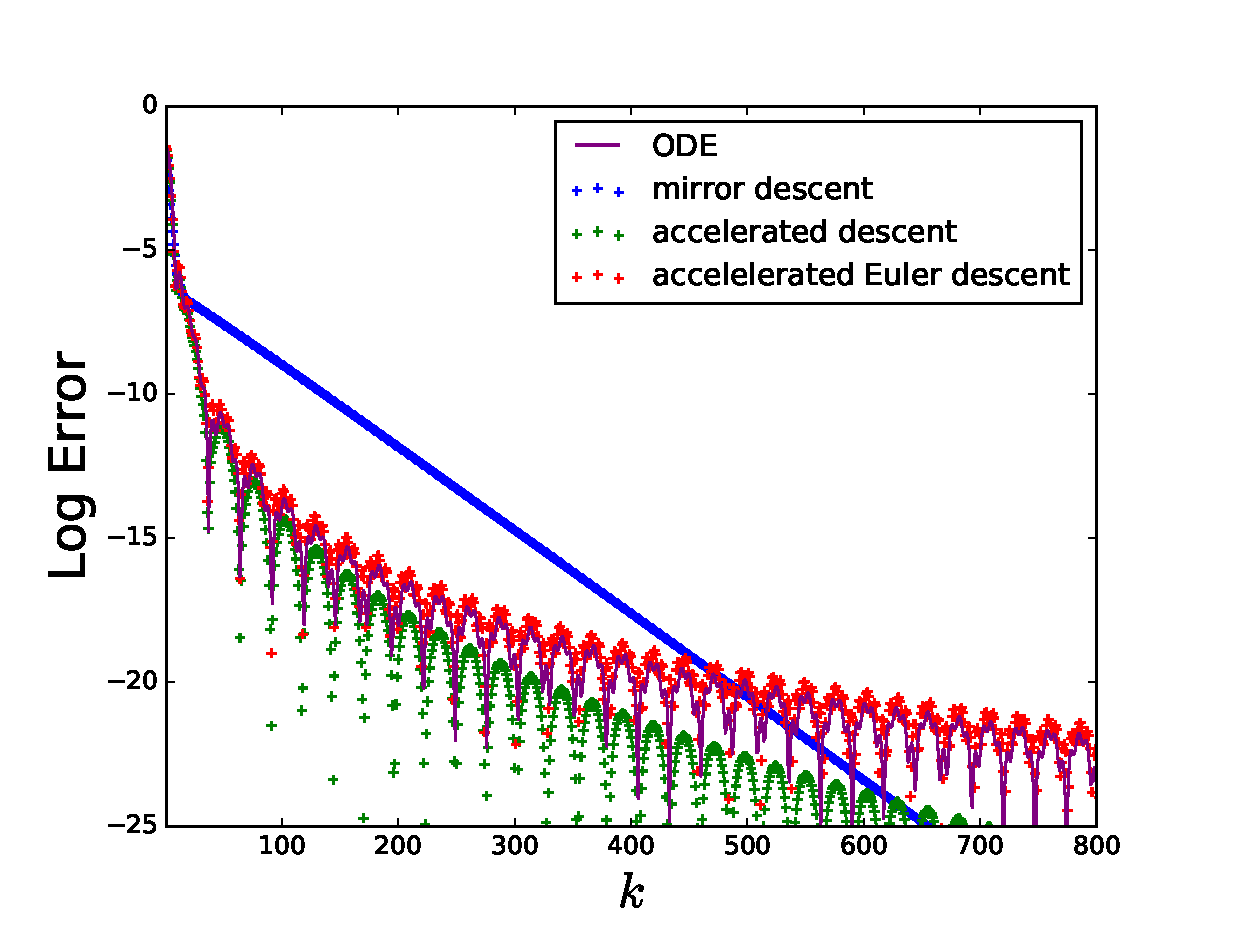
\includegraphics[width=1\linewidth]{Experiments/amd-quadratic-logerror.eps}
\caption{Error of $f-f^*$ vs iteration number for the auadratic objective}
\label{fig: quaderr}
\endminipage\hfill
\minipage{0.48\textwidth}%
 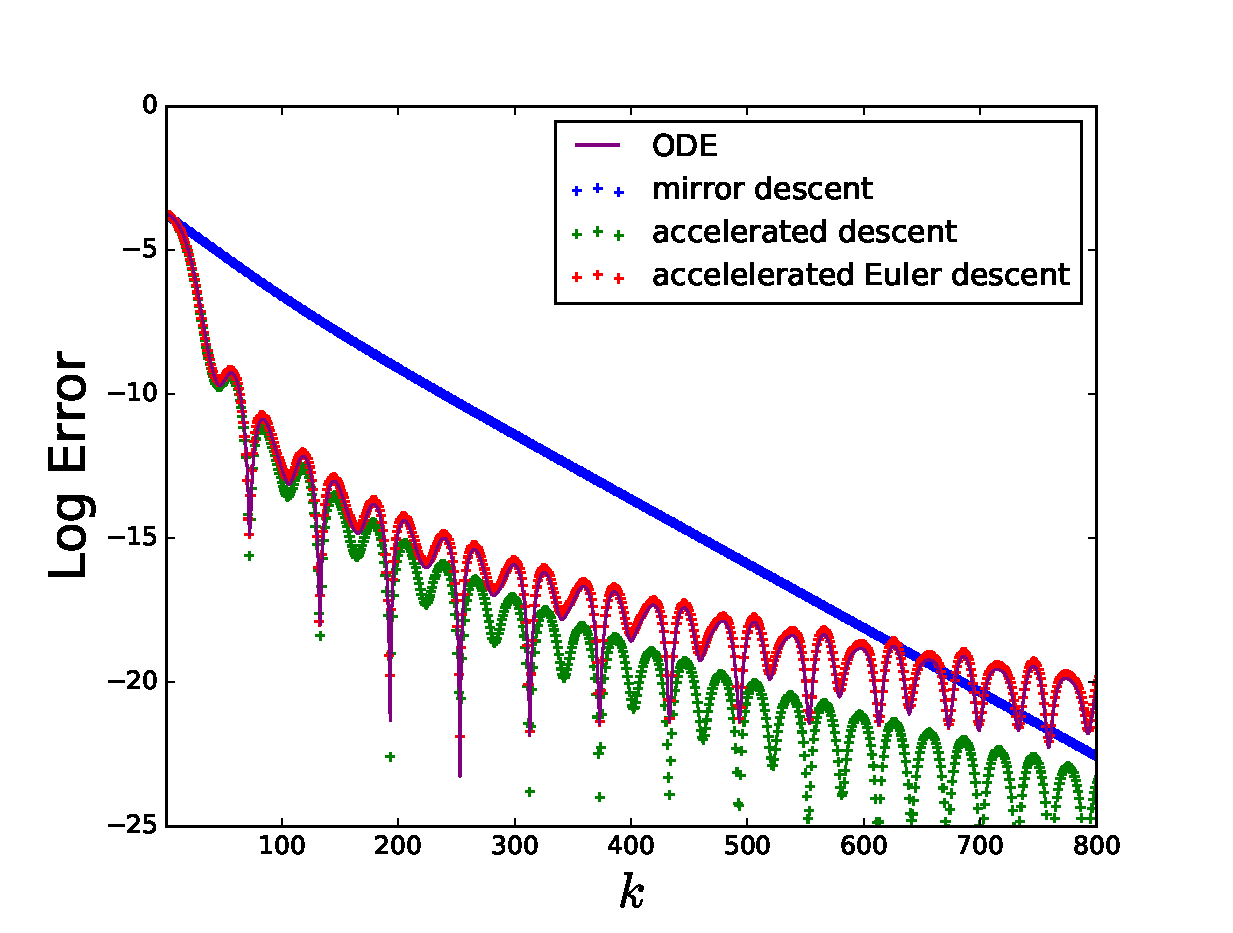
\includegraphics[width=1\linewidth]{Experiments/amd-logsumexp-logerror.eps}
\caption{Error of $f-f^*$ vs iteration number for the log-sum-exp objective}
\label{fig: logsumexperr}
\endminipage
\end{figure}

\begin{figure}[!htb]
\minipage{0.48\textwidth}
  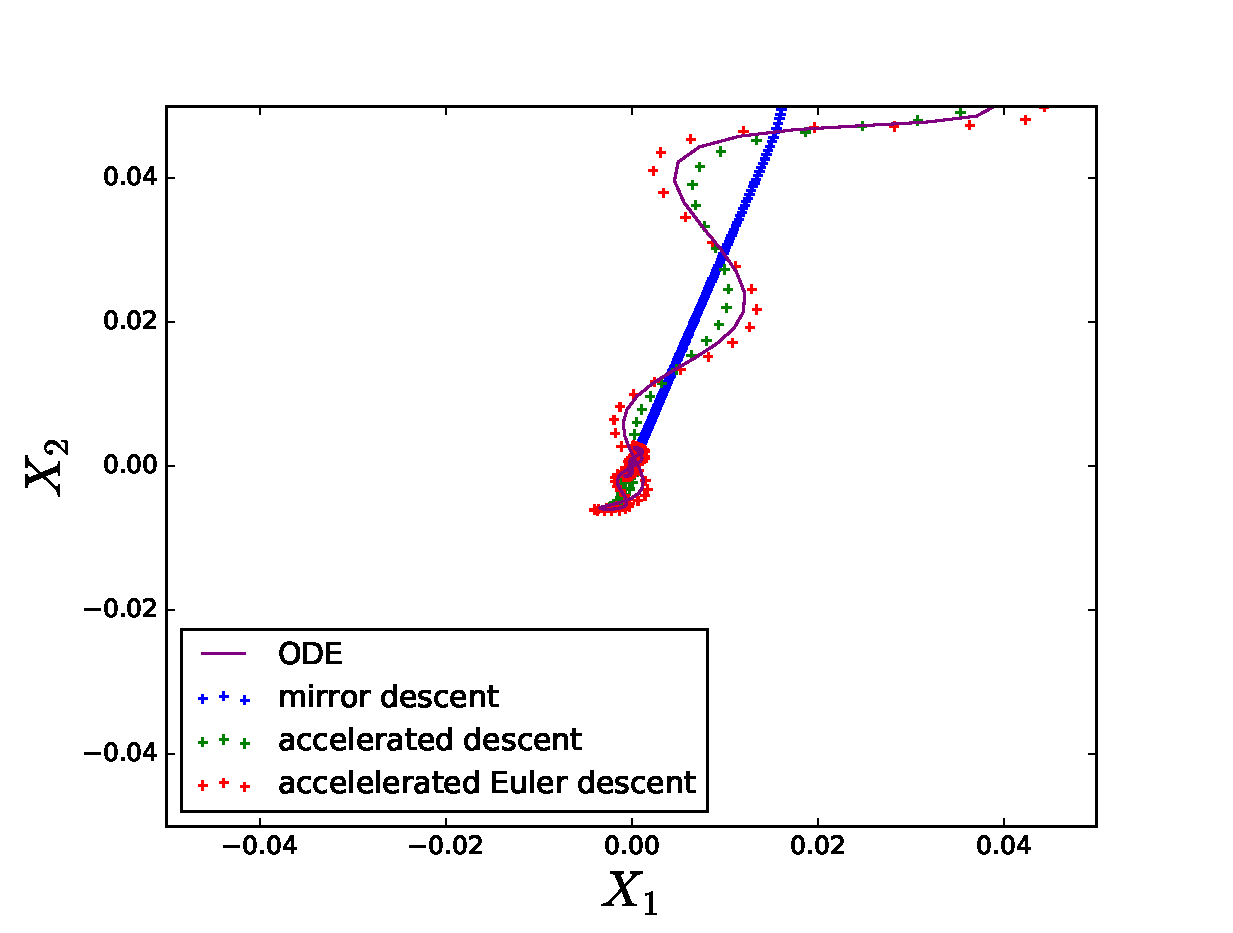
\includegraphics[width=1\linewidth]{Experiments/amd-quadratic-paths.eps}
\caption{Solution paths of $X(t)$ for the quadratic objective}
\label{fig: quadpath}
\endminipage\hfill
\minipage{0.48\textwidth}%
 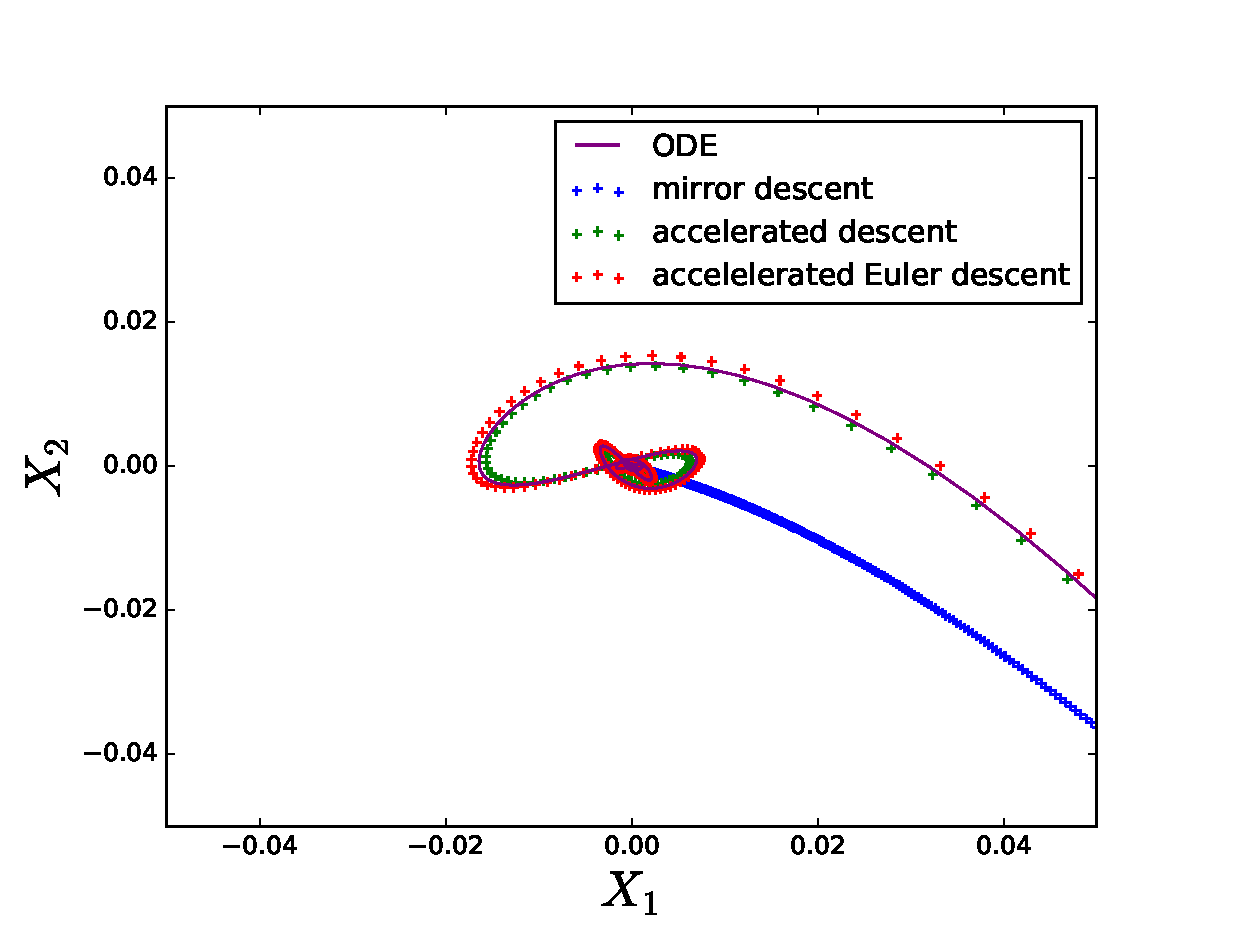
\includegraphics[width=1\linewidth]{Experiments/amd-logsumexp-paths.eps}
\caption{Solution paths of $X(t)$ for the log-sum-exp objective}
\label{fig: logsumexppath}
\endminipage
\end{figure}